\section{Problem 1: MORPHOLOGICAL PROCESSING}\label{problem-1-morph-process}
A binary image, \textbf{sample1.png}, is given in Figure 1. Please implement several morphological operations and provide discussions about the results. (Note that the white pixels represent foreground objects and the black pixels are background.)

Given an image, \nameref{sample1}.

Original image \nameref{sample1} for question \nameref{problem-1-morph-process}.
\begin{figure}
    \centering
    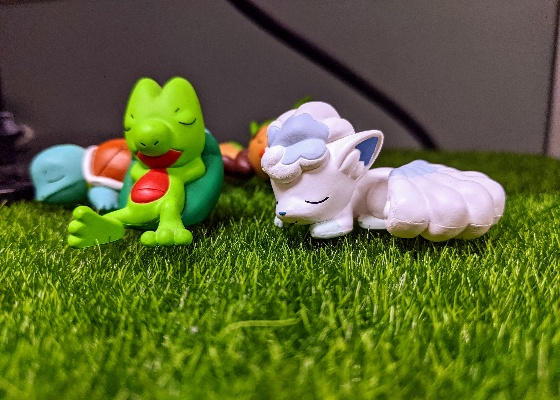
\includegraphics[width=0.7\textwidth]{src/sample1.png}
    \caption{\textbf{sample1.jpg}}
    \label{sample1}
\end{figure}

\subsection{(a)}\label{1_a}
Perform boundary extraction on \textbf{sample1.png} to extract the objects’ boundaries and output the result as \textbf{result1.png}.

\paragraph{Motivation}
Extract the boundary (or outline) of an object.
Recall of generalized \textbf{dilation} and \textbf{erosion} in \textit{Lec 4 page 32}.
\begin{itemize}
    \item dilation: \(G(j, k) = F(j, k) \oplus H(j, k) \)
    \item erosion: \(G(j, k) = F(j, k) \ominus H(j, k) \)
\end{itemize}
where \(H(j, k)\) is \textbf{structure element}.

\paragraph{Approach}
We could follow the formula in \textit{Lec 4 page 39}. The formula of \textbf{boundary extraction} is 
\[
    \beta(F(j, k)) = F(j, k) - (F(j, k) \ominus H(j, k))
\]
It is the original image \textbf{minus} its erosion.

I start from generalized \textbf{dilation} and \textbf{erosion}. This is my \alert{core function} for \nameref{1_a}, \nameref{1_b} \& \nameref{1_c}.
\begin{enumerate}
    \item Convolution with \textbf{structure element} \(H(j, k)\) to get \(T_{r, c} \{F(j, k) \} \) .
    \item Conduct \textbf{erosion} or \textbf{dilation}:
	\begin{itemize}
	    \item \textbf{erosion}: \(G(j, k) = \cap_{(r, c) \in H} T_{r, c} \{F(j, k) \}  \) \\
		As we \textbf{intersection} of all \(T_{r, c}\), we could check the \textbf{sum of matching} \(T_{r, c}\) is \alert{equal} of \# \(1\) in \(H_{j, k}\).
	    \item \textbf{dilation}: \(G(j, k) = \cup_{(r, c) \in H} T_{r, c} \{F(j, k) \}  \) \\
		As we \textbf{union} of all \(T_{r, c}\), we could check the \textbf{sum of matching} \(T_{r, c}\) is \alert{greater than} \(0\).
	\end{itemize}
\end{enumerate}
This approach is transform \textbf{intersection} \& \textbf{union} as \textbf{convolution with condition}.

Then conduct the \textbf{boundary extraction} by formula. 
\begin{enumerate}
    \item Design the \textbf{structure element} \(H(j, k)\) as well as \textbf{origin points}.
    \item Calculate \textbf{erosion} \(F(j, k) \ominus H(j, k) \)
    \item Obtain \textbf{boundary extraction}.
\end{enumerate}

\paragraph{Performance of results}
In the end, I choose same \textbf{structure element} in \textit{Lec 4 page 39}, that is
\[
    H(j, k) = \begin{bmatrix}
	1 & 1 & 1\\
	1 & 1 & 1\\
	1 & 1 & 1
    \end{bmatrix}
\]
with \textbf{center point as origin}.

Result of problem 1(a): \nameref{result1}.
\begin{figure}
    \centering
    \includegraphics[width=0.7\textwidth]{src/result1.png}
    \caption{\textbf{result1.jpg} Boundary extraction}
    \label{result1}
\end{figure}

\paragraph{Discussion}
I try some different \textbf{structure element}.

\textbf{Different of structure element}:
\[
    H(j, k) = \begin{bmatrix}
	0 & 1 & 0\\
	1 & 1 & 1\\
	0 & 1 & 0
    \end{bmatrix}
\]
\alert{TBA}...
\[
    H(j, k) = \begin{bmatrix}
	1 & 1 & 1\\
	1 & 0 & 0\\
	1 & 1 & 1
    \end{bmatrix}
\]
\alert{TBA}...

\textbf{Different size of structure element}:
Size \(H_{5 \times 5}(j, k)\)
\alert{TBA}...

\subsection{(b)}\label{1_b}
Perform hole filling on \textbf{sample1.png} and output the result as \textbf{result2.png}.

\paragraph{Motivation}
Given a pixel inside a boundary, hole filling attempts to fill that boundary with object pixels.

First, this operation uses \textbf{dilation}(\(\oplus \)). We could reuse the core function designed in \nameref{1_a}. But I find out the result is not good as my expectation.

Second, as we could treat it as \textit{Fill tool in Painter}, we could use \href{https://leetcode.com/problems/flood-fill}{flood fill} algorithm for this problem.

\paragraph{Approach}
My idea is start from \textbf{breadth-first search (BFS)}. The idea comes from \href{https://leetcode.com/problems/flood-fill/discuss/1086688/Python-BFS-easiest-Soln}{LeedCode discussion}.
\begin{enumerate}
    \item Initialize empty queue and add the \textbf{start point} to fill.
    \item Scan the color of position \((i, j)\)
	\begin{itemize}
	    \item if the current is not visited \&
	    \item the color of current is the same as queue of the start point.
	\end{itemize}
	We fill the new color of this pixels.
\end{enumerate}
I use the trick that start from the \textbf{top-left corner pixel} with \textbf{black}. And fill up all \textbf{background} as \textbf{tag} (\(2\) ). Then I keep it as background and replace other pixels with \textbf{white color} (\(255\) ).

\paragraph{Performance of results}
In the end, I choose the \textbf{flood fill} algorithm.

Result of problem 1(b): \nameref{result2}.
\begin{figure}
    \centering
    \includegraphics[width=0.7\textwidth]{src/result2.png}
    \caption{\textbf{result2.jpg} Hole filling with flood fill}
    \label{result2}
\end{figure}

\paragraph{Discussion}
We could follow the formula in \textit{Lec 4 page 41}. The formula of \textbf{hole filling} is 
\[
    G(j, k) = ( (G_{i-1}(j, k) \oplus H(j, k) ) \cap F^{c}(j, k) ) \cup F(j, k)
\]
where \(i=1, 2, \dots \), \(F^{c}(j, k)\) means the \textbf{complementary} of original image.
It is the \textbf{interior} of original image \textbf{union} with \textbf{boundary}.

My approach is
\begin{enumerate}
    \item Calculate complementary \(F^{c}(j, k)\)
    \item Dilation then \textbf{intersection} with complementary \( (F(j, k) \oplus H(j, k)) \ast F^{c}(j, k) \) \\
	As we just get \(\{0, 1 \} \) of dilation as well as complementary results, we could times (\(\ast\) ) them as \textbf{intersection}.
\end{enumerate}
Moreover, I add parameters of \textbf{\# repeated} of hole filling operations.

Give the same \textbf{structure element}
\[
    H(j, k) = \begin{bmatrix}
	1 & 1 & 1\\
	1 & 1 & 1\\
	1 & 1 & 1
    \end{bmatrix}
\]
with \textbf{center point as origin}. And repeat hole filling with \textbf{12} times.

Here is the result: \nameref{result2_lec4}
\begin{figure}
    \centering
    \includegraphics[width=0.7\textwidth]{src/tmp/result2_lec4.png}
    \caption{\textbf{result2\_lec4.jpg} Hole filling in Lec 4 page 41}
    \label{result2_lec4}
\end{figure}

Although \nameref{result2} shows we successfully fill all holes, it expands original objects and connect to each other. 
Why does it occur? I consider that my approach is not as good as \textit{Lec 4 page 41}. As I don't choose the \textbf{interior points} in the objects. So all objects become larger and larger.

\subsection{(c)}\label{1_c}
Please design an algorithm to count the number of objects in Figure 1. Describe the steps in detail and specify the corresponding parameters.

\paragraph{Motivation}
Scan an image and groups its pixels into components based on pixel connectivity.

First, this operation uses \textbf{dilation}(\(\oplus \)) again. We could reuse the core function designed in \nameref{1_a}. However, I can't count the number of objects as I don't calculate it \textbf{iteratively}.

Second, I use \textbf{two-stage scan} for couting the number of objects. The detail steps is shown below.

\paragraph{Approach}
My approach is
\begin{enumerate}
    \item Initialize the object with tag \(-1\).
    \item Scan the \(8\)-neighbors of object \(F(j, k) \neq 0\) as \texttt{G\_subarray}.
	\begin{itemize}
	    \item if there are two above tags in \texttt{G\_subarray}, we store it as \textbf{connected cluster}.
	    \item else substitute the new cluster tag for \(-1\) or propogate existed tag in \texttt{G\_subarray}.
	\end{itemize}
    \item Get \texttt{label\_object\_adj\_mat} from \textbf{connected cluster}.
    \item Check the connectivity of label object adjacency matrix by \(A^{k}\). \\
	where \(k\) is number of clusters (candidate label objects).
    \item Merge the connect clusters as final label objects. And count it!
\end{enumerate}

\paragraph{Performance of results}
I use the \nameref{result2} than count it!

Result of problem 1(c): \nameref{prob1c_cluster} with \(20\) objects.
\begin{figure}
    \centering
    \includegraphics[width=0.7\textwidth]{src/tmp/prob1c_cluster.png}
    \caption{\# 20 Objects with color}
    \label{prob1c_cluster}
\end{figure}

\paragraph{Discussion}
We could also conduct it for \nameref{result2_lec4}.
Result of problem 1(c): \nameref{prob1c_cluster} with \(11\) objects.
\begin{figure}
    \centering
    \includegraphics[width=0.7\textwidth]{src/tmp/prob1c_cluster_lec4.png}
    \caption{\# 11 Objects with color (Lec 4)}
    \label{prob1c_cluster_lec4}
\end{figure}

